\documentclass[12pt,twoside,a4paper]{report}
\usepackage{graphicx}
\usepackage[numbers]{natbib}
\begin{document}
\title{GUI for mail-merge using Erlang and Erlguten}
\author{Yuan Zhiqian}
\date{April 2011}
\maketitle
\cleardoublepage
\begin{abstract}
  Klarna AB is a financial company which provides payment solutions for the e-commerce sector, and they need to generate a lot of invoices everyday, which involves a large amount of tedious work, so they need a tool to facilitate this task. The new method of invoice generating consists of two sub-process, i.e. designing templates and make mail-merging between templates and userdata。

  This project aims for implementing a system to solve the issues described above, it mainly targets on the mail-merging of templates and userdata, besides it also provides a prototype of GUI for designing the templates. The final goal is to realize the automation of invoice generating to the greatest extent, later in this report I will illustrate how far this goal is reached.

  This system involves many technique areas, the techniques mainly used are Erlang, Erlguten, Cappuccino framework, javascript, rubyonrails etc.
\end{abstract}

\cleardoublepage

\listoffigures
\cleardoublepage
\tableofcontents

\chapter{Introduction}
  This chapter introducts the project by generally describing it and giving its background. At the end of this chapter, the report structure is shown.
\section{Project Overview}
  Invoice generating is always a big task for companies, finacial companies especially. The problem is not only the huge amount of the generation, but also the series of problems aroused during the procession of this repeative and tedious task. Typoes may occur, and a lot of time are wasted on the repeative inputting of data for every individual invoices. So it is always good to make this kind of task automated. However, automation has its own disadvantage, that is, the lack of human-maintaining leads to the potential flaws in typesetting, layout designing etc. So the programmer has to consider the issues which were formerly faced by marketing people who design invoices by hands. 

  Fortunately there's a tool called erlguten which we can use to help achieve the goals in typesetting, so that tasks like space management, auto-linebreaks of paragraphs are no more big issues. The question becomes how to design the system so that it can make good use of erlguten's functionality, together with its own mail-merging fucntionality, as well as to achieve the full automation from the template designing to PDF generating.

  This project is developed using many languages. The backend batch program is implemented in Erlang/OTP, and the GUI is implemented using Cappuccino framework, which is written in Objective-J, a super-set of Javascript. And the whole system is packed and connected using RubyonRails, which can be used to implement web services easily. 

  The project is maintained using git, the repository is homed on github. You can find the project and download the codes in this link: 

  https://github.com/yuanzhiqian/mailmerging\_using\_erlang\_and\_erlguten

  This report is edited using Latex typesetting software.

  During the development of this project, engineer and managers in Klarna AB has been helping me a lot with various issues. I would like to express my great appreciation to Erik Stenman who has been guiding me and prompting valuable advices, and Samir Fors who has recommended me the brilliant javascript-based web application framework -- the Cappuccino framework, and many other developers for their help. 

\section{Background}
  In this background section, two aspects will be described: the thesis background, and the technical background.
\subsection{Thesis Background}
  This thesis is initiated and sponsored by Klarna AB.

  Klarna AB is a fanancial company which provides payment solutions for the e-commerce sector, during the daily transaction, invoice generating appears to be a heavy task so it is good to make this process automated. The company is using "Klarna Online", an in-house developed system written in Erlang, to generate transaction documents. The origianl system let the marketing people manually write Erlang codes to design the layout of invoices, with the help of erlguten, which is very incovenient and what is worse is that the end users have to know a lot of technical details to be qualified for this work. Besides, according to their plan, in the invoices, transpromos\cite{transpromo} need to be added as well, so now they want an improved system to replace the old one, so as to alleviate the burden of invoice generating and realize the transpromo functionality. The following goals are supposed to be achieved by the new system:

\begin{enumerate}
\item The marketing and product development departments should be able to do most of the maintenance of the document templates. (i.e. The invoice generating task is divided into two parts -- templates maintenance, and the batch of mail-merging and pdf generating, the latter is supposed to be fully automated and the former is supposed to be facilitated by providing intuitive GUI for template designing and maintaining. )
\item The system should support functionality for Transpromo and making more attractive transaction documents.
\end{enumerate}

\subsection{Technical Background}
\subsubsection{Erlguten}
  Erlguten is a system for hiqh quality typesetting, ErlGuten is free soft-ware. ErlGuten aims to produce typographic quality PDF directly from XML or from a program.\cite{erlguten03}
 
  Here is a short citation from the official introduction:

\begin{quote}
  ErlGuten is designed for the production of large and complex documents
with complex layout requirements, like newspapers or books. In ErlGuten
layout, content, and document management are considered separate issues.
Layout is template based - Content is assumed to be stored as a large num-
ber of documents in a file system or data base, document management is con-
sidered as a mapping operation which takes documents in the content data
base and maps them onto templates to produce hight quality output.\cite{erlguten03} 
\end{quote}

  Erlguten provides a bundle of methods in "pdf" module (In the new version of erlguten, the module is renamed as eg\_pdf, and some functionalities from other modules are combined into this module.), using which, the programmer can specify the layout of a pdf document and it then will be generated into pdf file by invoking the export method that erlguten provides. Erlguten also provides text and image management, which have greatly simplified the process of typesetting. 

  Besides of those described above, erlguten also defines its own typesetting formats and syntax, the user can specify layouts separately in a xml file, on the other hand, the contents are written in another xml file, with the "layout to be used" indicated, then the erlguten will do the batch for those files and generate the final pdf. The aim of this is to separate layout of a document from the contents.

  At the beginning, I adopted this functionality because during the batch process, erlguten will do the text management automatically; but later, because of the new requirements, this method has to be discarded, and I decided to directly use pdf module for pdf generating. However, the old library for the original version of my project is retained for potential uses, although the methods, which rely on that library, are deprecated. 

\subsubsection{Cappuccino Framework and Objective-J}
  Cappuccino Framework\cite{capp} is an open source framework for developing web applications that look and feel like Mac OS desktop applications. Cappuccino provides handy APIs which programmer can use to directly develop web applications without needing to concern themselves with HTML, CSS or even DOM. 

  Cappuccino is implemented using a new programming language called Objective-j, which is analogous to Objective-C in some way, like message calls etc, but it is built on Javascript and its compiler is totally written in Javascript, so programs written in Objective-j don't need any server side compilation. Objective-j inherits some design patterns from Cocoa, like delegation etc.

  Cappuccino framework provides Cocoa-like API, so that Mac OS X programmer can easily get hand on this framework.  

\section{Report structure}
  The following parts of this report will be arranged as follows:

  First the issues faced and the goals to achieve will be specified, then in the Implementation chapter, the system's structure is shown and each component is described. The Evaluation chapter will show the result of tests on the system to see how well the problems are solved. And I will state the future works to be done on improving the mail-merging component and extending the GUI prototype. Finally I'll make a summary on the project.

\chapter{Problem Description}
  This chapter first describes the issues faced, then it will describe the goals and motivation. At the end, I will specify the method I use.

\section{Issues}
  The automation of invoice generating involves many aspects, so there're a lot of thing I need to do research on. 

  First, the company uses mail-merging to achieve automation, that means it's hard to use erlguten's original pdf-generating method, because they follow different logics. Second, I need to define the format of templates by myself, and I also need to consider the conversion from GUI elements to xml-based template files. The third, as the company requires, a GUI is preferred, but because of the limitation of time, it is hardly possible to build such a sophisticated GUI from scratch. So what I need to do is to try to find a framework to facilitate the work. 

  The mail-merge and pdf generating is the main functionality of this project. And there're many fractions needed to be considered too. One of the tricky issues is the calculation of page count. Because there are tables and lists in the invoices, and their length is expanding according to the user data, so we need to determine the page count so as to chose correct template for them. 

  Besides of these, I also need to think about how to combine every components and make the whole system run on good condition -- if everything works perfect, the end user should see nothing more than the GUI itself, so they may not expect something like a exclamation saying that "an error occurred, templates are not in the right directory", those confusing internal errors do exist when trying to make every individual components cooperate with each other.

  Moreover, how to make the GUI intuitive and convenient to use is also a big issue, although it is not mandatory to provide a fully-functioning GUI, but it is always good to at least bring up some good ideas in the prototype. 

  And there are some requirements on the functionalities to implement as well, which will be described in the next section.

\section{Goals and motivation}

  Because the requirement of automation, the system adopts mail-merging technique. Along with the requirements from Klarna company, the goals are as follows,

\begin{itemize}
\item Implement the mail-merging functionality which can replace dynamic fields in the templates with specified user data.
\item The system should be able to deal with text, image, table and list items.
\item The system should be able to estimate the length of document, and select the right template among the alternatives.
\end{itemize}

\section{Method Used}
  Mail-merge technique is adopted to make the system dynamically process large amount of user data. To mark up a dynamic field, I introduce escape characters. I use "\#" to indicate a dynamic field. During a mail-merging process, the system checks the template file, extracts dynamic fields(also called as "parameter") from the template, and make a query in the user data files. The system then substitute the field with the actual data it finds, or send out an error message in case the parameter's name can't be found in user data files. 

  The mail-merge of text and image are performed in the same way, i.e. replace the parameter with the actual data found in the user data files. As for image, the data would be the path where images are stored.

  As for tables and lists, things are different. There are two reasons, first of all, table and list need to follow special format and layout; second, a table item is dynamically expanding, you never know how many rows are needed until you access the user data files. However, the aim of automation is to let the user not have to know about the actual user data, because only the program needs to access the user data. So in the template, a table is simply indicated as a table item, with some information of formats and a index referring to the table data in the user data files to present. So the mail-merge of a table item is done in this way: the system find out the table items, and check its name, then the system look up this name in the user data files. When they system finds the right data, it concatenates the data with the format information in the template file, this merged segment will later be process by the PDF generation module, in that phase, indicated columns will be chosen to print and format information, if any, will be parsed and performed on the printing procedure.

  The list is easier to process, because no dynamic-length lists are required, we just need to define the items of lists in the template file, and replace those items in the same way as dynamic texts.

  The GUI is implemented based on cappuccino framework, it is a outstanding tool to design web applications. The GUI is built from a tutorial provided by a website\cite{tut}, so it inherits a lot of the original layouts of the tutorial. The GUI allow users to create as many templates as they want(but due to some restrictions, the amount of templates may be limited below three. This will be explained in the next chapter), the users edit the template as if they are using painting board, now the GUI allows the users to draw frames to indicate the boundaries of items, if time allows, I may add the functions of editing view so that the user can type in contents and attributes in the frame, in the future's work, some auxiliary tools like rulers and coordination tags may be provided to aid the alignments. When the users finish editing, they can generate xml files for the templates by pressing the corresponding button, when everything is ready, the user can press the generate pdf button to export pdf files. This function is done by making a call to the back-end modules, i.e. the parts described above.

\chapter{Implementation}
  This chapter describes the technical solution of this system. 
\section{System Environment}
\begin{itemize}
\item Ubuntu Linux 10.10
\item Erlang R14B02 (erts-5.8.3)
\item Erlguten 
\item Cappuccino framework 0.9
\item Javascript
\item RubyonRails 3.0.7
\end{itemize}
\section{System Structure}
  Figure \ref{fig1} illustrates the system structure in graphics. As described in figure \ref{fig1}, the user data are first retrieved from database and automatically converted into XML files, but this process is done outside of the system. Then the marketing people design templates according to the requirements using the GUI running in the web browser. By pressing the "save templates" button, the templates will be sent to the server by making an XMLHttpRequest\cite{XHR}, which will be processed by the web service written in rubyonrails. When this is done, the user would like to generate pdfs, and he will press "generate pdf" button to send another XMLHttpRequest, when the server receive the request, it will execute the script to call the mail-merge functions and do the mail-merge, generating invoices as pdf files. 

\begin{figure}[p]
\centering
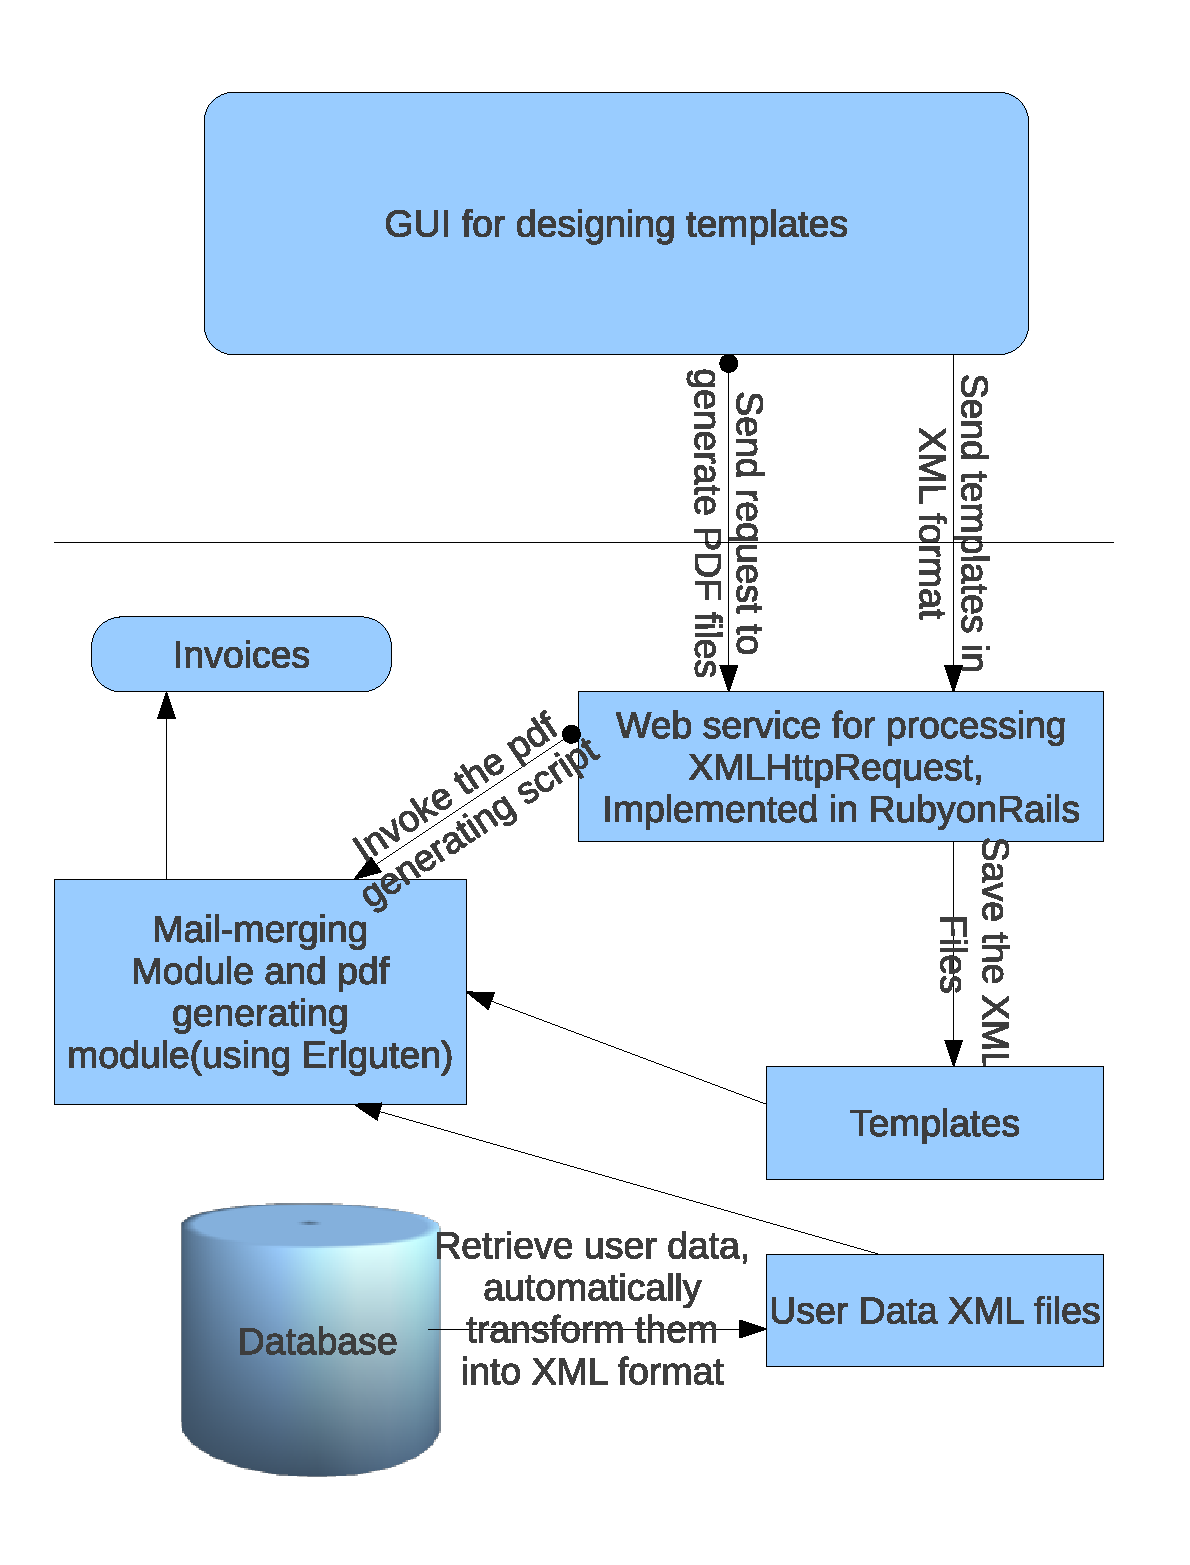
\includegraphics[scale=0.5]{systemstructure.eps}
\caption{System Structure illustrated in graphic form}
\label{fig1}
\end{figure}

\section{Implementation for each part}
\subsection{Template Format}
  I would like to use a sample to explain the format of template:

\begin{quote}

$<$?xml version="1.0" ?$>$
$<$template count = "3" alt2 = "N/A" alt3 = "N/A"$>$
$<$paper name = "first" class = "front"$>$

  $<$frame name = "trademark" class = "img" x = "48" y = "30" width = "94" height = "20" grid = "true" bg = "default" font = "N/A" fontsize = "N/A" paraIndent = "N/A" maxlines = "N/A" continue = "N/A" break = "N/A"$>$\#tm$<$/frame$>$

  $<$frame name = "hello" class = "text" x = "48" y = "140" width = "177" height = "127" grid = "true" bg = "1.0,0.0,0.0" font = "Times-Roman" fontsize = "15/20" paraIndent = "0" maxlines = "4" continue = "none" break = "true"$>$Hello \#name, here is your invoice, this is a new version of template.$<$/frame$>$

  $<$frame name = "shoppinglist" class = "list" x = "48" y = "280" width = "177" height = "140" grid = "true" bg="default" font = "Times-Roman" fontsize = "14/20" paraIndent="0" maxlines = "30" continue="none" break="true"$>$

\{ul\}\{li\}\#first\{/li\}\{li\}\#second

\{/li\}\{li\}\#third\{/li\}\{/ul\}$<$/frame$>$


  $<$frame name = "shoppingtable" class = "table" x = "48" y = "450" width = "177" height = "100" grid = "false" bg="default" font = "Times-Roman" fontsize = "12/24" paraIndent="0" maxlines = "30" continue="shoppingtable2" break="true"$>$

\{table columns = \{goods, count, price, place\}\}

\{tr\}\{th\}\#goods\{/th\}\{th\}count\_col?\{/th\}

\{th\}\$price?\{/th\}\{th\}place\{/th\}\{/tr\}\{/table\}$<$/frame$>$

$<$/paper$>$

$<$paper name = "second" class = "middle"$>$
  
  $<$frame name = "trademark" class = "img" x = "48" y = "30" width = "94" height = "20" grid = "true" bg = "default" font = "N/A" fontsize = "N/A" paraIndent = "N/A" maxlines = "N/A" continue = "N/A" break = "N/A"$>$\#tm$<$/frame$>$

  $<$frame name = "shoppingtable2" class = "table" x = "48" y = "140" width = "177" height = "640" grid = "false" bg="default" font = "Times-Roman" fontsize = "12/24" paraIndent="0" maxlines = "30" continue="shoppingtable3" break="true"$>$

@shoppingtable$<$/frame$>$

  $<$frame name = "faq" class = "text" x = "300" y = "128" width = "280" height = "153" grid = "true" bg = "default" font = "Times-Roman" fontsize = "12/24" paraIndent = "0" maxlines = "6" continue = "none" break = "true"$>$Question and Answer: \#text$<$/frame$>$

$<$/paper$>$

$<$paper name = "third" class = "end"$>$
  
  $<$frame name = "trademark" class = "img" x = "48" y = "30" width = "94" height = "20" grid = "true" bg = "default" font = "N/A" fontsize = "N/A" paraIndent = "N/A" maxlines = "N/A" continue = "N/A" break = "N/A"$>$\#tm$<$/frame$>$

  $<$frame name = "shoppingtable3" class = "table" x = "48" y = "140" width = "177" height = "400" grid = "false" bg="default" font = "Times-Roman" fontsize = "12/24" paraIndent="0" maxlines = "30" continue="none" break="true"$>$

  @shoppingtable2$<$/frame$>$

  $<$frame name = "slip" class = "img" x = "0" y = "550" width = "600" height = "250" grid = "true" bg = "default" font = "N/A" fontsize = "N/A" paraIndent = "N/A" maxlines = "N/A" continue = "N/A" break = "N/A"$>$\#slip$<$/frame$>$

$<$/paper$>$

$<$/template$>$ 

\end{quote}

  As you may notice, there are three "paper" nodes under the root node "template". But this is not always the case, it would take many words to explain this: basically, an invoice consists of trademarks, text contents, tables, graphic elements and a slip to indicate the payment details, and the slip is supposed to be always placed at the end of the document. And an invoice always has a table as well, but the length or the table is not sure of when the marketing people designs the templates, so the number of pages needed is unknown too, therefore they should prepare three kinds of templates to cover all the cases that may occur -- they are: one-page template, to be used for the documents that only have one page (the slip is at the bottom of the page); two-page template, to be used for the documents that only have two pages (the slip is at the bottom of the last page); three-page template, to be sued for the documents that have more than two pages (the slip is at the bottom of the last page, and there's also a "middle page template" to define the pattern of the pages between the front page and the end page). 

  And because that the template may be one-page template, two-page template, or three-page template, there should be attributes to indicate the alternative templates if the current template doesn't fit. So the "template" node contains "alt2" and "alt3" attributes for this use.

  In each "paper" node, there are many frames. Currently there are four kinds of frames: text frame which denotes a flow of normal texts, and image, table, list frames which denotes the corresponding items. The type of frames are specified by the "class" attribute. The attributes of frame is listed as follows:

\begin{itemize}
\item name, the name of frame
\item class, the type of frame
\item x, the x coordinate of the top left corner of frame
\item y, the y coordinate of the top left corner of frame
\item width, the width of frame
\item height, the height of frame
\item grid, whether or not the grids are needed to be shown
\item bg, the background color of frame
\item font, the font of texts in the frame
\item fonsize, the size of texts in the frame
\item paraIndent, the indent of paragraphs
\item maxlines, the number of lines needed
\item continue, deprecated attribute
\item break, deprecated attribute
\end{itemize}

  The content of four kinds of frames are as follows:

  \textbf{text}: the content of a text frame node contains static texts as well as dynamic texts. The dynamic texts are denoted beginning with a \# mark. A sample of the content is like this: 

  $<$frame .... $>$ Hello \#name, the amount you need to pay is \#price $<$/frame$>$

  \textbf{image}: the content of a image frame node contains a parameter, which is to be replaced by a string which indicates the path where image files are stored, the replacement happens during mail-merge process. The parameter is just a dynamic text. This is a sample of a image frame:

  $<$frame .... $>$ \#trademark $<$/frame$>$

  \textbf{table}: the content of a table frame node is defined in a special format. Here is a sample of a table frame:

\{table columns = \{goods, count, price, place\}\}

\{tr\}\{th\}\#goods\{/th\}\{th\}count\_col?\{/th\}

\{th\}\$price?\{/th\}\{th\}place\{/th\}\{/tr\}\{/table\}

  As you may have noticed, the format of a table is very similar with that in HTML language, however I just borrow the idea from HTML and there're some differences between them. First a table has column attribute to indicate the columns selected to print out, because there may be many columns in a table in the user data files, and different template may want different columns to show, that's why we need such an attribute here. And a \{tr\}\{/tr\} couple denotes one row in the table, however, here it is only used to contain the table headers. Because some tables may have no headers, and some tables may have headers with different names, thus I decided that the user should be able to explicitly specify the headers. 

  \textbf{list}: the content of a list frame node is like this:

\{ul\}\{li\}\#first\{/li\}\{li\}\#second\{/li\}\{li\}\#third\{/li\}\{/ul\}

  The format of list definition is also borrowed from HTML language, just using different marks. The content of list is also dynamic texts, its substitution method is the same as described above. 
  
\subsection{Mail-merging and pdf generating algorithm}
\subsubsection{Overview}

  The mail-merge and pdf generating functionality is the main component in this system, figure \ref{fig2} shows the flow of this process. As is shown in the figure, the system first read in template file and user data file, and transform them into erlang term form, then the system call the preprocess function to calculate the number of pages needed and chose the proper template. The rule is, if more than 3 pages are needed, then a 3-page template, which includes front, middle and end page template, is chosen; if 2 pages are needed, then a 2-page template, which contains front and end page template, is chosen; if only one page is needed, then a 1-page template, which only has front page template, is chosen. I need to point out that the current template has a higher priority, which means if the current template is proper, then it is selected. For example, if a 3-page template is used, but the total pages needed are 2, then this 3-page template is still chosen. 

  There are two internal records defined to store the template information, after the preprocessing, these internal data structures are created, then the mail-merge procedure is started. After the mail-merging, the data is parsed once again to generate internal data structure for frames. Then the generatePDF function is called. 

  During the pdf generating part, the system first examine each frame's type, and then call the corresponding function in the text\_img\_table\_list module to generate pdf stream for them. The table and list may expand up to many pages, that's why we do the preprocess to determine the number of pages needed. If a table occupies many pages, then a 3-page template is used, and usually there would be some texts and images in the middle pages as well, so after print out each page, the system will examine that page again to print other frames in that page. 

  When it comes to the final page, the end-page template is used and invoice slip is printed.

  This is the general workflow of the system, next I will describe each part in detail.

\begin{figure}[p]
\centering
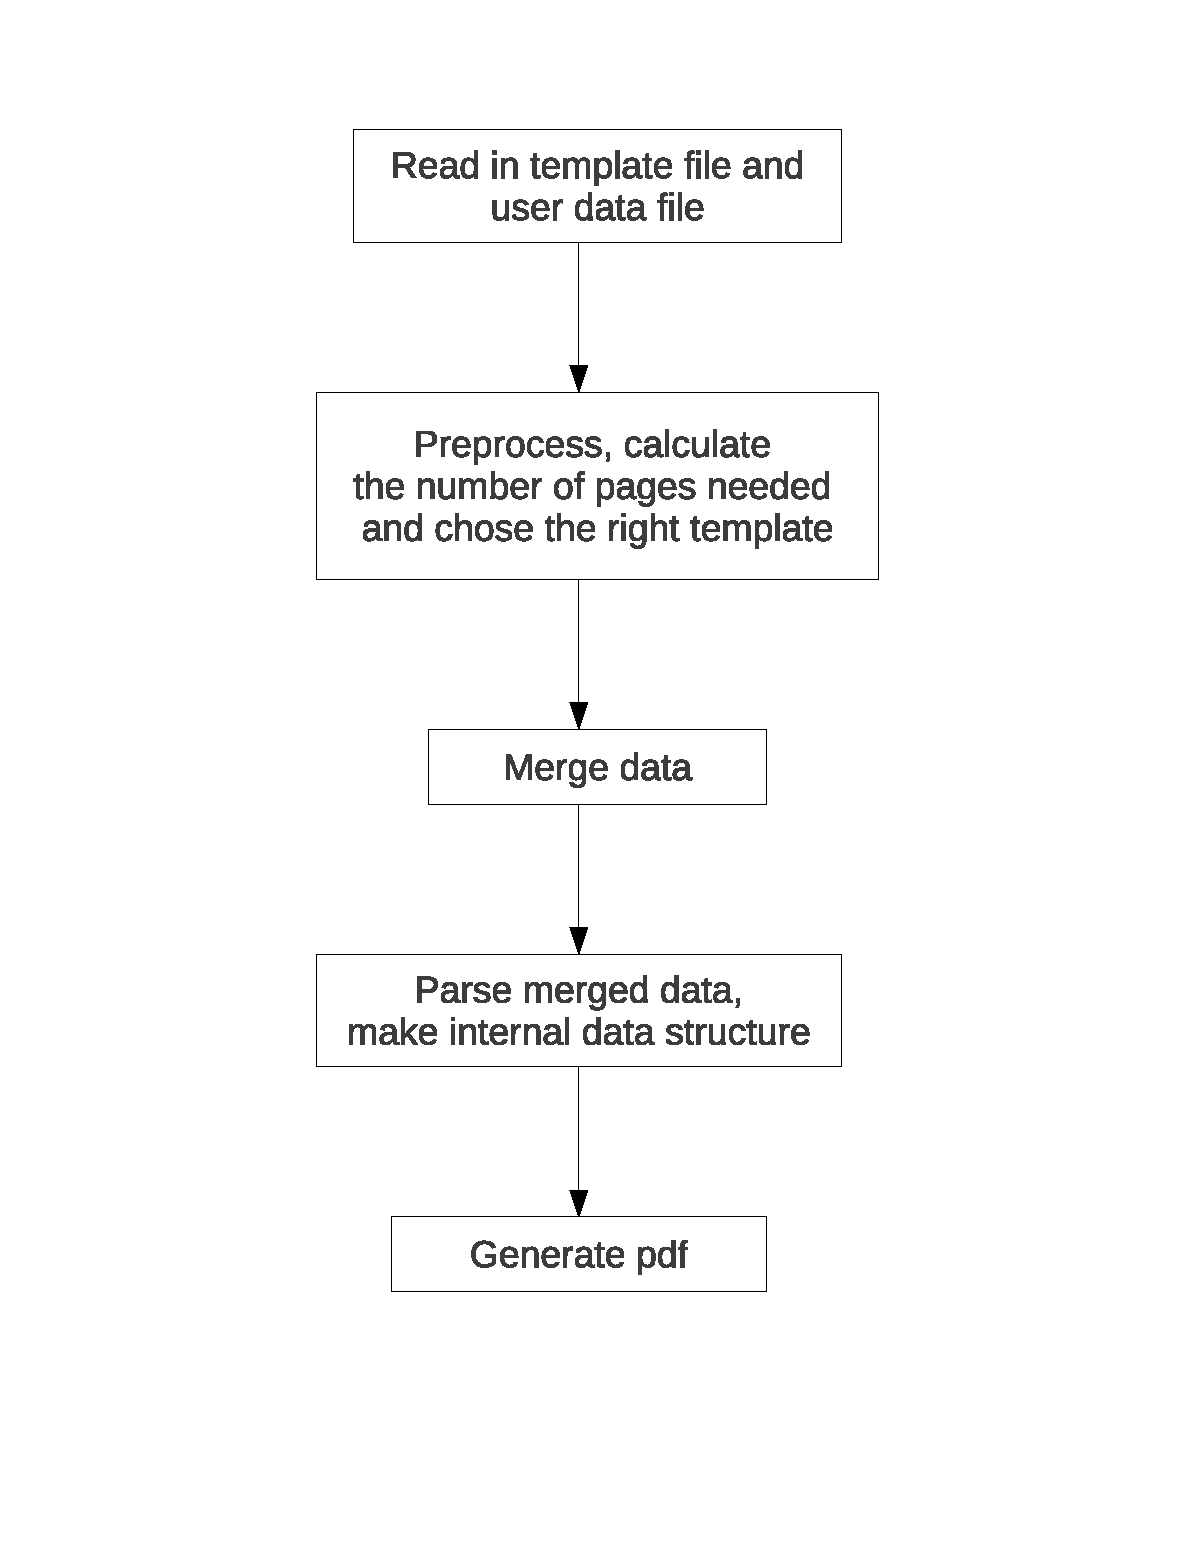
\includegraphics[scale=0.5]{mailmergeprocess.eps}
\caption{Flow chart of mail-merge process}
\label{fig2}
\end{figure}

\subsubsection{Preprocess}

  During the preprocess part, the proper template is chosen and the number of papers needed is calculated. The template chosen algorithm is, first check the current template, if it is a 3-page template, then it is selected directly; else if it is a 2-page template, then check if the number of pages exceeds 2 -- which is done by calling overThreshold2. 

  The algorithm of overThreshold2 is, check each tables in the "front page" template, calculate the length of them and calculate the "bottom limit" as well, the "bottom limit" the top of the frame which comes immediately after the table item -- since a table is not supposed to cover any other frames in the same page. Then the bottom of table is compared with the bottom limit of the front page, if the bottom of table exceeds, that means the table will run down to the next page, so we need to compare its bottom with the bottom limit of the end page, to compare them, we need to first find out the "continue table", which shows the position where the extension of the table will be set to, the bottom of the "continue table" is compared with the bottom limit of the end page. If it exceeds again, that means more than 2 pages are needed, in this case, the alternative 3-page template is selected.

  If the current template is 1-page template, then we need to first check if more than one page is needed by calling overThreshold1 function, the algorithm is similar to overThreshold2, so I won't describe again; if only one page is needed, then the current template is chosen, otherwise overThreshold2 is called to check if more than 2 pages are needed, if not, then the alternative 2-page template is chosen, otherwise the alternative 3-page template is chosen.

  This is the template chosen algorithm.

  Next the pages\_needed function is called to calculate the number of pages.

  Because in the template chosen process, we only need to care about the two threshold, "one page" and "two pages", so we didn't really calculate the pages, instead we only check if any table exceeds the bottom of pages. So in the page calculation process, we can not reuse the functionality of template chosen, we need a different algorithm.

  The calculation of pages is like this, first we need to know that we need to calculate pages only when the template is a 3-page template. Suppose now the selected template is a 3-page template, we need to first calculate the bottom limits for the front page and the end page, which is the same as described above, then find the continue table in middle template, and find the continue table in end template. Now we have the position of continue tables in middle page and end page, next we calculate how many pages are needed in the middle pages -- we don't need to calculate the front page and the end page since they are simply a single page. Then we calculate a temporary page count by divide the total length of pages with 842, which is the length of an A4 paper. The "total length" of pages is achieved by this: ((842 - BottomLimit1) + (842 - BottomLimit2) + TableBottom), I need to explain a bit on this expression: it is not easy to understand but you can treat the expression in this way -- 842-BottomLimit1 is the height of "slip" (if any) in the front page, and 842-BottomLimit2 is the height of "slip" in the end page, TableBottom is acutually the top position of a table added with the length of table. So this expression is the addition of 1. The top of table, 2. the height of slip in the front page, 3. the length of table, 4. the height of the slip in the end page.

  But the addition described in the last paragraph is not the actual "total length", because the continue tables in the middle page and end page don't always start from 0. So we need to add the "height of blanks" as well. That's why I calculate the temporary page count first, we need to update the table bottom by adding the "height of blanks", so we have another expression: NewTableBottom = TableBottom + (NewMaxPages\_Temp - 2) * Y\_con1  + Y\_con2. Y\_con1 is the top position of continue table in the middle page, and Y\_con2 is the one in the end page. And now we can calculate the real page count by calling the function realMaxPages, it first update the page count with this expression NewMaxPages = ceiling(((842 - BottomLimit1) + (842 - BottomLimit2) + TableBottom) / 842), but this is not the final result, why? Because if the NewMaxPages is larger than the original one, that means more pages are needed than expected just now, if so, we need to add the "height of blanks" of those new pages as well, and update the table bottom once again, then re-calculate the page count. Thus this is an iteration: calculate the page count -- compare with the original page count -- update the new table bottom -- re-calculate the page count. Finally, the page count doesn't increase any more, that's the final result. 

\subsubsection{mail-merge}

  Before the mail-merge starts, the system checks the template type, and then make mail-merge for each page in the template. The mail-merge is done frame by frame, if there's any frame in the template containing fields which don't exist in the data file, the system will print out a error message. The mail-merge is processed differently on the four type of frames, for text, image and list frames, the system substitute the dynamic fields with the data found in the data file; for table frames, the system attach user data with the table format information in the template. The substitution of dynamic fields is like this: first the system check the fields beginning with a hash (\#) mark, using a regular expression "\#[a-zA-Z0-9\_]+", then the system finds out all the fields beginning with two hash marks -- which means a normal string with a hash mark, and those normal strings are removed from the match list, so that the dynamic fields are filtered, then the system looks up those fields in user data file, and replace them with the real data. 

  There's one special type of frame, which is the so-called "continue table" frame. Its usage is describe the position of the "continue table", which is the extension of the tables in prior pages. Those frames' content is a table name beginning with a "@" mark, which indicates the table it succeeds to. Meanwhile, this "continue table" is also referred to in the "continue" attribute of the original table. During the mail-merging process, there's nothing happening on this kind of frames.

\subsubsection{pdf Generating}
  
  The process of pdf generating is like this: first the system examine the frames in the front page, and call the corresponding functions to print them, if there're table frames in the front page, the system will automatically add pages if the tables require more pages to display. And the system also print out the other frames in those pages every time it about the change pages, when it comes to the end page, the system will check the end page template, and print out necessary slip etc on the page. 

  The project borrows some concept as well as functions from erlguten, because its functionalities of typesetting is quite sophisticated. Proper adjustments are done to make sure the system can work well with those erlguten functions.

  Some tables have headers, so the first task of table printing is to process the headers, and after the headers are printed, we should consider whether the next row runs onto the next page, in order to do so, we check the space left on the page to see if it is enough for another line, if no, a new page is added. And on the new page, the table is positioned according to the attributes of "continue table" frame in middle/end page template. 

  Then the content of tables are printed, when it comes to the bottom of page, a new page is added and the table is positioned according to the corresponding "continue table" frames, which is the same as described above.  

\subsection{GUI Implementation}

  The GUI is implemented using Cappuccino framework\cite{capp}. I have reused the codes from a tutorial provided by a cappuccino tutorial website\cite{tut}, so the GUI inherits its layout and looks like a painting board. The GUI allows the end users to design templates without using any erlang code, the WYSIWYG characteristic of the GUI makes the template design much more convenient and intuitive. However, due to the limited time, this GUI is temporarily a prototype, but it can be easily extended without needing to make too much effort. 

  Cappuccino framework allow programmers to make MAC OS-like web applications, and its programming language, objective-j, inherits much of the concepts from Cocoa. 

  There's not too much needed to explain on the implementation details, but I'd like to illustrate the infrastructure of this GUI, so that people who wants to extend this prototype can get a clear clue. 

\begin{figure}[p]
\centering
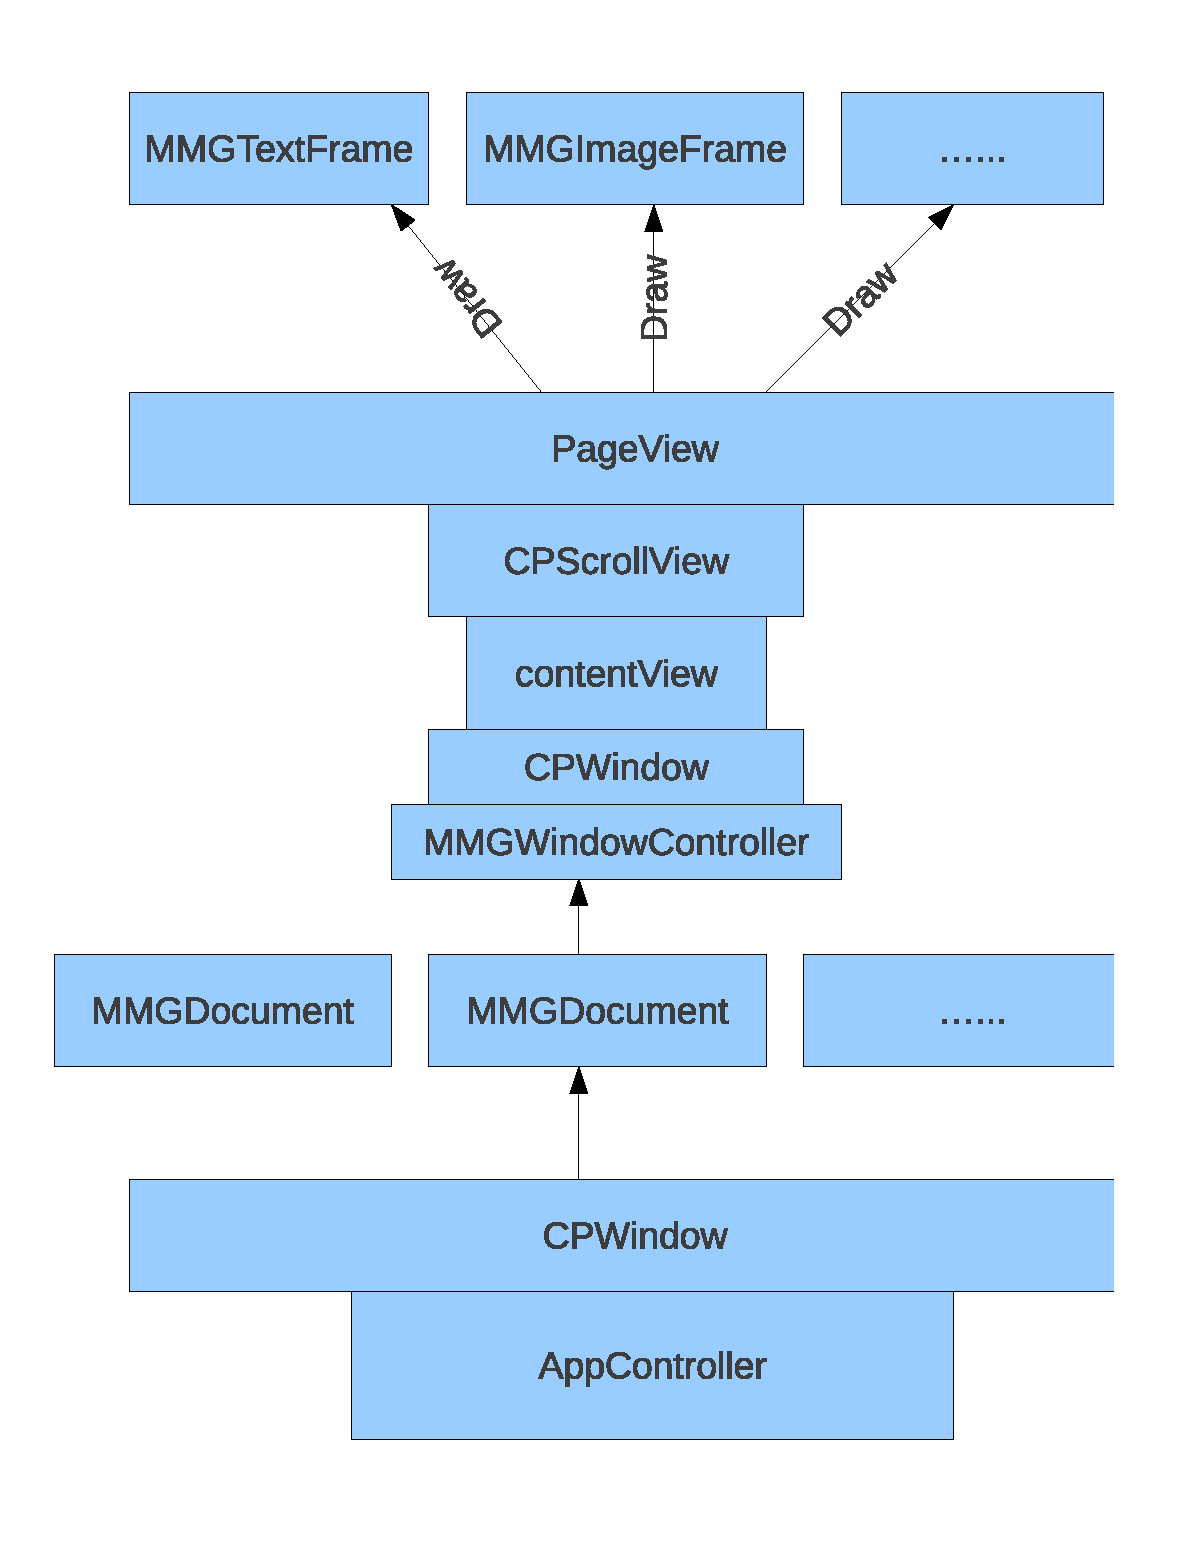
\includegraphics[scale=0.5]{GUIInfrastructure.eps}
\caption{The infrastructure of GUI}
\label{fig3}
\end{figure}

  As the figure \ref{fig3} shows, the GUI starts from AppController, which initializes a CPWindow -- in Cappuccino framework, such a window is the browser window itself, which is analogous to the screen in a desktop application. The GUI starts with one MMGDocument object, which inherits the CPDocument class, it is the "model" in MVC design pattern. By pressing the buttons in the window, users can create more MMGDocument object, which stands for the pages in a template, and are presented as separate floating windows. According the the current specification of template, only up to 3 MMGDocuments are allowed, and they stands for the front, middle and end page templates respectively. 

  A CPDocument initializes a MMGWindowController, which controls a bunch of window -- this window is different with the window mentioned above, it is actually analogous to the windows in a desktop application. And the window contains a content view, which contains more views. I add a scroll view to show the full content of the page, and then add a page view into the scroll view. In the page view, mouse events are captured and processed, so that users can draw frames and move them around. Users can also edit the frames and delete them -- which is not currently available and is to be done as the future work.

  Frames inherits the MMGGraphic class, which is borrowed from the original tutorial. It is just a general data model, and is extended into different frame types, with more information added.

  This is basically how the GUI works. In the next sub section, I will describe how the GUI is connected and communicate with the other components in the system.

\subsubsection{Template Generating}
 
  When the user press the "save templates" button, the saveTemplates function is called. And the template generating process is started. The template is stored in xml format, so we need to convert the internal representation of template data into DOM\cite{dom}. This process is done in the packXml function. The system process every document object and generate one "paper" node for each document object. The final template will be made up of several "paper" nodes, in those nodes, frame nodes are defined -- following the same structure as describe earlier in this report. 

  After the template is translated into DOMs, the system serializes the DOMs into XML string, and send it in the body of an XMLHttpRequest, the XML string will be received and processed at the back end, which will be described later.

\subsection{Combination of GUI and back-end system}

  The system consists of 3 major parts, namely GUI, back end Web service, and the mail-merge module. 

  The GUI is written in Objective-J, and it is a superset of javascript, its communication with web server is through so-called "XMLHttpRequest", which allows a web application to update with web services without needing to refresh the current page. 

  The web server is written in RubyonRails, which is a handy framework that can be used to easily implement a web service. Although currently I just use the very basic functionalities provided by RubyonRails, but its powerful scaffolding can be used in the future to make the system more intact. 

  The mail-merge module is all written in Erlang code, and uses erlguten lib to generate pdf files. This module is connected with the GUI via the web service described above, when the user press "generate pdf" button, another XMLHttpRequest is sent, and when the web server receives the request, it will run the script to call the functions in mail-merge module. 

\chapter{Evaluation}
  
  Many tests are made to evaluate how well the system works. During the tests, many problems occurred and were fixed one by one. But at present the tests are still based on some hard coding method, because the editing view of GUI is left for the future work, so it is a pity that we can not show the actual work flow of a complete system. It is still a prototype.

  But the mail-merging module is complete, and it is also the most critical component required by the company. So I made a lot of test on this component.
  
\section{Mail-merging}
\subsection{Text}

  The substitution of dynamic texts works well, the system can extract dynamic fields correctly, and look up those fields in the user data, make proper substitution. The system can also distinguish between dynamic fields and static fields that starts with a hash mark. 

  The system automatically breaks one paragraph of text into several lines, according to the width of the text frame. 

  Besides, the users can also set different background colors, or require to print out grids for the texts. Those functionalities also work fine.

  Users can specify various fonts for the texts as long as the system supports, and they can also specify the size of text, but too large size may cause error during the printing of texts, and may results to a blank frame printed out which can be really confusing. The reason is erlguten examines the boundary of "boxes" (which is converted from frames), if the texts are so large that the boxes can not hold them all, then instead of printing out part of the texts, erlguten simply skips the current frame and does't print out any texts at all. So the users should estimate the potential size of texts, and make proper frames, I should say this is not user-friendly design, maybe in the next version this situation would be changed. 

\subsection{Image}

  The image adding is successful, but the users are required to provide the width and height of images, this may be not so convenient. I think a better solution can be made in the future's work.

\subsection{Table}

  The process of tables is also considered as a big task of this project. Because tables have expanding length, and we need to add pages automatically and put the continue tables in the proper position etc. The test turns out to be very successful, the system can calculate the page count precisely, and the tables are printed normally. The users can also specify which columns are needed to be shown, and this functionality also works fine.

\subsection{List}

  There's not too much to say about the list, although it has a special format, its mechanism is almost the same as dynamic texts. The tests' results look fine, the only flaw is that I haven't found a way to print out bullets for list items, but it is not a big issue.

\section{GUI}

  The GUI is a prototype at present. And I reused the codes from a Cappuccino tutorial to build this GUI, the GUI provides frame drawing and translation functionalities, the XML file generating and client-server communication is also available. The GUI also supports multi-document editing. However more auxiliary tools are expected to make this GUI a convenient tool.

\section{Web service test}

  To make the whole system intact, the web service takes major responsibilities like processing XMLHttpRequests, template file storage, path problems and script executing. 

  During the tests, I realized the prominent issue is the path problems. Because in a system, different components have different environments, and they may all treat its current path as the default path, which may cause the path dis-accord problems. Because those problems are not obvious, it is always frustrating to coordinate the path among various components. So I made a adjustment, instead of using path+filename pattern in the parameters, I manage path separately, this adjustment works perfectly as expected, and the path problems seem to be solved.

\chapter{Future work}

  This project is a master thesis project which is carried out in a few months. Because of the limited time as well as experience and technical limits, there are many flaws and unhumanizing designs to be fixed and improved in this system. Also, as described in earlier chapters, the GUI is implemented as a prototype, so there are surely a lot of extensions that can be made on this GUI.

\section{Mail-merging part}

  There are several inconvenient designs in the mail-merging component, which are listed as follows, together with the modification expected for the future work.

\begin{itemize}

\item As described earlier, the template designers have to estimate the size of potential texts and make proper text frames, and confusing errors may occur if the frames are not large enough for the contents. This is not user-friendly. Because commonly a template is supposed to be used for various of users, and this error may only happen in some of the user files. It is very inconvenient for the template designers to modify the templates just for some specific users. So a more fault-tolerant design may be like this: when the system finds that the current text frame is not large enough, it first calculate the spaces available on the page to see if those spaces can be used to contain the texts, and then gives the template designers a warning of this situation, then make a suggestion to enlarge the frame temporarily to contain the flow of texts; however if the there aren't enough spaces left, then the system may tell the template designers that the error is hard to fix, and suggest he/she to provide a alternative template.

\item At present the lists are printed as rows of items, there are no bullets printed at the beginning of each row because I haven't found a way to do so. This may be fixed in the future as well.

\item Now the height of rows in tables are specified in template files, but the width of columns is temporarily hard coded in the program, this should also be fixed in the future. 

\item The text may also occupy more than one page, but currently this situation is not considered to reduce the complexity. In the future work, this should be fixed as well.

\item It is expected that texts can be added onto images, so that dynamic fields in an invoice can be printed at the blanks of the images. I haven't handle this issue yet, so this is also postponed into the future work.

\end{itemize}

\section{GUI part}

  Since the GUI is now a prototype, so there are a lot of things that can be added and improved.

\begin{itemize}

\item Add editing view functionality, so as to allow the designers to edit frames' content as well as set their attributes. 
\item Add coordinate displaying functionality, so that designers can estimate the space usage. 
\item Add alignment lines, this auxiliary tool is very helpful when you want to keep frames aligned in a row or make their center at the same line etc. The idea is show alignment lines when the frames are moved to a position that its top is aligned with other frames' top, etc. And to make it more user-friendly, the frames should be automatically align when users move them to the neighborhood of the position where they are aligned with other frames.
\item Defined different frame types.
\item Add rotation functionalities.

\end{itemize}

  Those are what I can image so far, but the future work of this GUI is of course not limited to those ideas. More improvements can be made according to the needs of daily usage.

\section{Others}

\begin{itemize}

\item Some aesthetic works can be done to make the invoice printed look more sophisticated.
\item The "front page" can have more pages actually, this can be done by pdf merging. 
\item I haven't check with the transpromo designers, maybe some more functions are required to make it easier to add transpromo functions. 

\end{itemize}

\chapter{Summary and Conclusions}

  This project is dedicated to improve the efficiency of commercial invoice generating by using mail-merge methodology. And it also prompted a way to design templates by implementing a prototype of GUI which can be extended in the future according to the practical requirements. 

  In this project I made research in typesettings and solved problems like table length calculation and table flow arrangement, and good effects are achieved. I also made research on erlguten and get inspired from its design pattern to define the template format that is used in my project. The template format definition experienced many versions, and gradually evolves into the current style. There may still be some defects in the template format definition but it seems to fit most of the cases. 

  I also made research on GUI designing, because this project is supposed to be web-based, so I gave up the idea to use Java. Before I was recommended with the powerful Cappuccino framework, I also made research on the hacking of openoffice using python script, but those methods all proved to be inconvenient. I also checked JQueryUI and Raphael library, but they are for interactive web page implementations instead of web application. Finally I chose Cappuccino framework, and it proves to be very suitable for web applications development.

  Except for the GUI ends up to be a prototype, this project kind of achieved the expected goals. More future works are still needed to make it a useful tool, but since the structure of the system is cleared illustrated, it shouldn't be very hard.

  At the end of this report I would like to express my acknowledgement to the people who helped me a lot during this project once again. 

\begin{thebibliography}{9}
\bibitem{erlguten03}Erlguten repo, 2003. Erlguten repository on google code. 

http://code.google.com/p/erlguten/

\bibitem{transpromo} Transpromo described in wikipedia.

http://en.wikipedia.org/wiki/Transpromotional

\bibitem{XHR} W3C Candidate Recommendation of XMLHttpRequest

http://www.w3.org/TR/XMLHttpRequest/

\bibitem{capp} Cappuccino website. 

http://cappuccino.org/

\bibitem{tut} Cappuccino tutorial website. 

http://www.nice-panorama.com/Programmation/cappuccino/

\bibitem{dom} W3C Document Object Model.

http://www.w3.org/DOM/

\end{thebibliography}

\end{document}
